
\documentclass[conference]{IEEEtran}
\IEEEoverridecommandlockouts
% The preceding line is only needed to identify funding in the first footnote. If that is unneeded, please comment it out.
\usepackage{cite}
\usepackage{algpseudocode}
\usepackage{amsmath,amssymb,amsfonts}
\usepackage{graphicx}
\usepackage{textcomp}
\usepackage{xcolor}
\usepackage{array}
\newcolumntype{M}[1]{>{\arraybackslash}m{#1}}


\def\BibTeX{{\rm B\kern-.05em{\sc i\kern-.025em b}\kern-.08em
    T\kern-.1667em\lower.7ex\hbox{E}\kern-.125emX}}
\begin{document}

\title{Latent Dissonance via Efficient Quantile Estimation}

\author{\IEEEauthorblockN{Eric Joraskie}
\IEEEauthorblockA{}
\and
\IEEEauthorblockN{Nick Kantack}
\IEEEauthorblockA{}}

\maketitle

\begin{abstract}
This whitepaper introduces a method of estimating the quantiles of a distribution that is observed in a stream fashion. Specifically, this method requires no queuing of data but instead updates the mean, variance, and quantile estimates as each datum is processed. We prove that this estimation algorithm is an unbiased estimator of the true statistics and has a time complexity that is linear in the desired quantile resolution.
\end{abstract}

\section{Mean Estimator}

When a queue of $N$ data points with mean $\langle x \rangle$ loses a datum ($x_{-}$) and gains a datum ($x_{+}$) the new mean $\langle x \rangle_{2}$ can be tracked via
\begin{align}
\langle x \rangle_{2} = \langle x \rangle + \frac{x_{+} - x_{-}}{N}
\end{align}
If we make the approximation that $x_{-}=\langle x \rangle$, we can obtain the unbiased estimator of the new mean $\langle x \rangle_{2}$ of
\begin{align}
\langle x \rangle_{2} \approx \langle x \rangle \frac{N-1}{N} + x_{+}\frac{1}{N}
\end{align}
This is a recognizable exponential moving average. Furthermore, $\langle x \rangle_{2}$ is a linear combination of data ($x_{+}$) each of which has an expectation of $\langle x \rangle$, therefore, the expectation of $\langle x \rangle_{2}$ is $\langle x \rangle$ by linearity of expectations, and thus we have an unbiased estimator.
\section{Variance Estimator}

Suppose that $\sigma^{2}$ is the variance before the data queue of the previous section loses $x_{-}$ and gains $x_{+}$. The new variance $\sigma_{2}^{2}$ is altered by three influences.
\begin{enumerate}
\item{The residual from $x_{-}$ is lost}
\item{The residual from $x_{+}$ is added}
\item{The residuals between the queue ends notice the change in mean}
\end{enumerate}
The first contribution is clearly $-(x_{-} - \langle x \rangle)/N$, and the second is clearly $(x_{+} - \langle x \rangle_{2})/N$. To find the third contribution, we examine the change in $\sigma^{2}$ induced by shifting the mean from $\langle x \rangle$ to $\langle x \rangle + \delta x$. Defining
\begin{align}
\widetilde{\sigma}^{2} = \frac{1}{N}\sum_{n=1}^{N}(x_{n} - \langle x \rangle)^{2}
\end{align}
and
\begin{align}
\widetilde{\sigma}^{2}_{2} = \frac{1}{N}\sum_{n=1}^{N}(x_{n} - (\langle x \rangle + \delta x))^{2}
\end{align}
we can solve for $\widetilde{\sigma}_{2}^{2} - \widetilde{\sigma}^{2}$.
\begin{align}
\begin{split}
\widetilde{\sigma}^{2}_{2} = \frac{1}{N}\sum_{n=1}^{N}\left(x_{n}^{2} - 2x_{n}\langle x \rangle + \langle x \rangle^{2}\right) + \\ \frac{1}{N}\sum_{n=1}^{N}\left(\delta x^{2} + \delta x \langle x \rangle - x_{n}\delta x\right)
\end{split}
\end{align}
\begin{align}
\widetilde{\sigma}^{2}_{2}=\widetilde{\sigma}^{2} + \delta x^{2} + \delta x \langle x \rangle - \frac{\delta x}{N}\sum_{n=1}^{N}x_{n}
\end{align}
\begin{align}
\widetilde{\sigma}^{2}_{2} - \widetilde{\sigma}^{2} = \delta x^{2}\tag{2}
\end{align}
Now we can combine all three changes to express $\sigma_{2}^{2}$ as a function of $\sigma^{2}$. Noting that $\delta x$ in this case $(x_{+} - x_{-})/N$ and thus
\begin{align}
\sigma^{2}_{2} = \sigma^{2} + \left(\frac{x_{+} - x_{-}}{N}\right)^{2} + \frac{(x_{+} - \langle x \rangle_{2})^{2} - (x_{-} - \langle x \rangle)^{2}}{N}
\end{align}
We can again applying the approximation $x_{-} \approx \langle x \rangle_{2}$ for an unbiased estimator of $\sigma_{2}^{2}$.

\section{Quantile Estimators}
Suppose that $n$ equally spaced quantiles ($q_{1},q_{2},...,q_{n}$) are to be estimated for the queue. We adopt an algorithm for updating the quantile positions stored in the vector $\boldsymbol{q}$. When a datum is observed which falls between two quantiles, the space between those two quantiles is reduced by a standard amount $s$ while the spaces between all other quantile pairs is increased by $s/(n+1)$ ($s$ is chosen to be small relative to $\sigma$, such as $s = \sigma / 10$). This is accomplished by the following rule.
\begin{align}
\begin{split}
q_{k} \leftarrow q_{k} - \frac{n-k}{n+1}s \ \text { if } \ x_{+} < q_{k} \\
q_{k} \leftarrow q_{k} + \frac{k+1}{n+1}s \ \text{ if } \ x_{+} \geq q_{k}
\end{split}
\end{align}
We can prove that under the condition described above, the resulting quantile are an unbiased estimator of the real quantiles of the queue. To prove this, we examine a specific, arbitrary quantile $q_{k}$. Let $P(x)$ be the unknown probability density function of the data. The expectation of the movement of $q_{k}$ after a new datum is
\begin{align}
\langle \Delta q_{k} \rangle = s \left[ -\frac{n-k}{n+1}\int_{-\infty}^{x_{k}}P(x)dx\ + \frac{k+1}{n+1}\int_{x_{k}}^{\infty}P(x)dx \right]
\label{integrals}
\end{align}
If all quantiles are correctly placed, then
\begin{align}
\int_{-\infty}^{x_{k}}P(x)dx = \frac{k+1}{n+1}
\end{align}
and
\begin{align}
\int_{x_{k}}^{\infty}P(x)dx = \frac{n-k}{n+1}
\end{align}
Substituting into \eqref{integrals}, we obtain
\begin{align}
\langle \Delta q_{k} \rangle = s \left[ -\frac{n-k}{n+1}\frac{k+1}{n+1} + \frac{k+1}{n+1}\frac{n-k}{n+1} \right]=0
\end{align}
Therefore, this serves as an unbiased estimator of the true quantiles.

\begin{figure}[!t]
\centerline{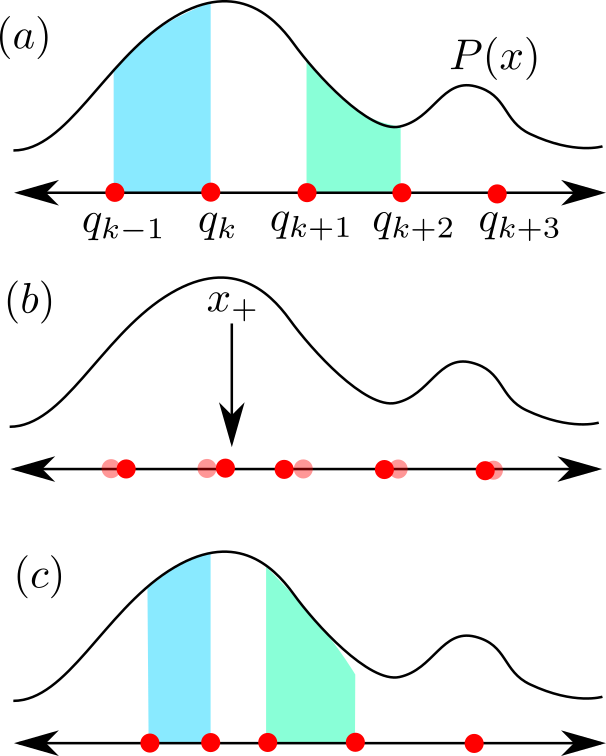
\includegraphics[scale=1]{figs/distributions.png}}
\caption{(a) Initially, the mean and variance are used to position rough estimates for the location of quantiles. These estimates will be incorrectly placed, and thus the populations between quantiles (blue and green regions) will be unequal. (b) When a new datum arrives, the immediate quantiles to either side are shifted inward by a small amount (e.g. $\sigma / 10$). Further off quantiles are also shifted inwards, although by an amount that scales down linearly with how many quantiles separate it from the datapoint. (c) In the steady state, quantiles will drift so that the populations between quantiles are approximately equal.}
\label{distributions}
\end{figure}

\end{document}